\section{My project}

\begin{frame}
\frametitle{My project}
My project has several parts:
\begin{itemize}
\item Given a terrain, automatically generate a road that minimizes a cost function based on slope and curvature.
\item Extending the wind simulator at the HPC lab to support meshes, e.g. roads through the terrain.
\item Import real world maps into the simulator.
\item If time, use snow height data from simulator as a part of the cost function when generating roads.
\item Also interesting: How is snow built up after it's removed from the road?
\end{itemize}
\end{frame}

\begin{frame}
\frametitle{Road generation}
I use the method described in Galin et. al.: Procedural road generation.
\begin{itemize}
\item Uses an A* search through the terrain, from a start to an endpoint.
\item Terrain is discretized into a grid.
\item Cost to go from gridpoint $\mathbf{p}_a$ to $\mathbf{p}_b$ is determined by a cost function.
\item Cost based on slope, curvature of the road, and length of the road.
\item Possibly soon: Also dependent on potential snow height.
\end{itemize}
\end{frame}

\begin{frame}
\frametitle{Real world maps}
Elevation maps from Kartverket is to be imported.
\begin{itemize}
\item Maps often come in the USGS DEM (US Geological Survey Digital Elevation Map) format.
\item An inconvenient format: Not a rectangular map, often skewed, space demanding (in ASCII)
\item These must be converted to a more reasonable format, e.g. a 16 bit RAW format.
\end{itemize}
\end{frame}

\begin{frame}
\frametitle{Real world maps}
\begin{figure}[ht]
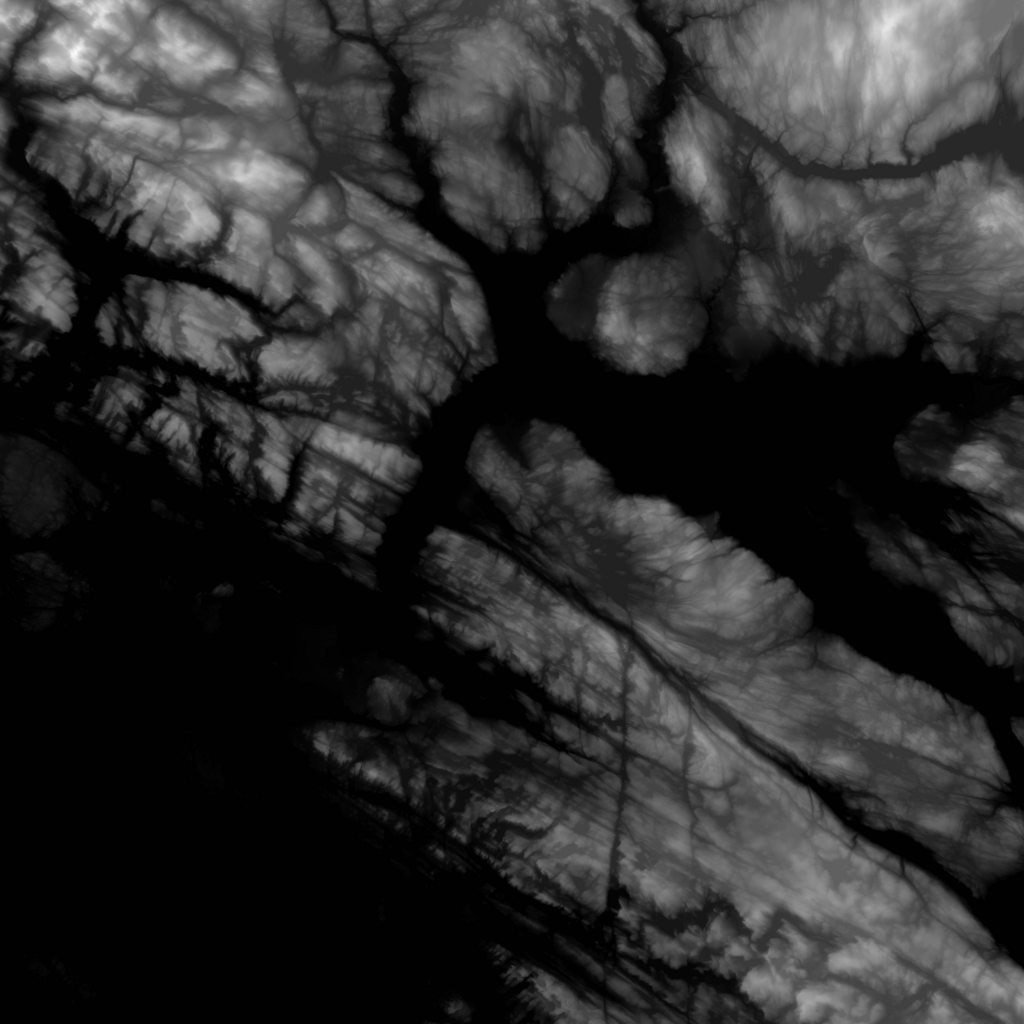
\includegraphics[width=0.75\textwidth]{gfx/converted_map}
\caption{Imported map}
\label{fig:trondheim}
\end{figure}
\end{frame}

\begin{frame}
\frametitle{Mesh support}
Currently, the only sort of models in the snow simulator is the terrain (Derived from a height map).
\begin{itemize}
\item At first, loading meshes into the snow simulator will be used to model roads.
\item Perhaps also famous landmarks for the real world terrains used (Space Needle in Seattle, Tyholt tower in Trondheim)
\end{itemize}
\end{frame}

\begin{frame}
\frametitle{Links}
\begin{description}
\item[Galin et. al.: Procedural road generation] \url{http://liris.cnrs.fr/~egalin/Pdf/2010-roads.pdf}
\item[Edissen: Utilizing GPUs for Real-Time Visualization of Snow] \url{http://www.idi.ntnu.no/\~elster/master-studs/robine/robin-eidissen-master-ntnu.pdf}
\item[Cvetanovic et. al.] \url{https://bioinformatics.cs.vt.edu/~guos/parallel/00205103.pdf}
%\item[A controlled clothoid spline] \url{http://imara.inria.fr/_media/users/franciscogarcia/a_controlled_clothoid_spline.pdf}
\end{description}
\end{frame}
